Some notions for Abelian groups will be helpful for understanding the relationships between class groups, quadratic number fields, and genera. Preliminary exercises:
\begin{ex}
Show that the direct product of cyclic groups $C_a \times C_b$ is cyclic iff $a$ and $b$ are relatively prime.
\end{ex}
\begin{proof}[Solution]
Write $C_a \times C_b$ as a lattice $(\mod a,\mod b)$ and pick any point on it (see Figure~\ref{cyclattice}). Then, the group operation on $C_a\times C_b$ is just moving one unit in each direction (and wrapping around where necessary).

If $a$ and $b$ aren't relatively prime, then $a = a'k$ and $b = b'k$, so the line created by repeatedly applying the group operation returns to its starting point after $a'b'k$ operations, but there are $a'b'k^2$ elements. Thus, only when $k=1$ (i.e. $a,b$ are relatively prime) is the product generated by one element and thus cyclic.
\begin{figure}[h]
\centering
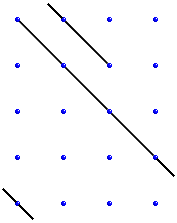
\includegraphics[width=2in]{cyclic}
\caption{A partial line through $C_{20} = C_4 \times C_5$.}
\label{cyclattice}
\end{figure}
\end{proof}
This statement is in fact equivalent to the Chinese Remainder Theorem (Theorem~\ref{crt}).
\begin{ex}
For a ``random'' Abelian group of order $n$, how often do the different types show up (e.g. $C_8$ versus $C_4\times C_2$ versus $C_2\times C_2\times C_2$)? Though this is a fuzzy question, it is possible to obtain an intuitive sense of the answer if not a concrete formula.
\end{ex}
\begin{defn}
A homomorphism from a group $G$ to a group $H$ is a function $f:G\to H$ such that $f(xy) = f(x)f(y)$.
\end{defn}
\begin{defn}
The kernel of a homomorphism $f$ is the set $\Ker f = \{x:f(x) = 1\}$.
\end{defn}
For example, on the group $\Z/p\Z \times \Z/q\Z$, then $f$ given by $x\to x^p$ has kernel $\Z/p\Z\times \{0\}$ (or the set of $(a,0)$ pairs). $f$ is only a homomorphism if the group is Abelian, since in general $(xy)^p = x^p y^p$ requires commutativity.
\begin{ex}[Cayley's Theorem]
Suppose $G$ is a finite Abelian group with order $k$ that divides some prime $p$. Show that some element of the group has order $p$ (i.e. that there is a cyclic subgroup with order $p$).

Hint: It will be helpful to consider $p$ elements of the group such that $\prod_{i=1}^p x_i = 1$ (e.g. $x_i= 1$ or $x, x^{-1}, 1, 1,\dots$, etc.). In particular, $y\cdot y\dotsb y =1$ if $y$ has order $p$. Then, count them in a way that considers order (relative, given by $a$ after $b$, or absolute, for permutations).
\end{ex}
%\begin{proof}[Solution]
%$G$ can be written as $G = C_{p^k} \times G'$, where $G'$ is some other Abelian group, and there exists an element of order $p$ in $G$ if there's one in $C_{p^k}$, since that element $a\in C_{p^k} \to (a,1)\in G$.

%Since $C_{p^k} \cong \Z/p^k\Z$, then the element corresponding to $p^{k-1}$ has order $p$ in $C_{p^k}$ and thus $G$.
%\end{proof}
\begin{cor}
The 2-torsion subgroup of a finite Abelian group (i.e. those elements that square to the identity) has size $2^k$ for some $k$.
\end{cor}%Which implies things about genera!
This implies things about the genera of reduced quadratic forms.
\begin{defn}
The principal genus is the genus of reduced quadratic forms that contains the identity element of the class group (i.e. either $x^2+ny^2$ or $x^2+xy+ny^2$).
\end{defn}
The principal genus is a subgroup of the class group $G$ given by $G^2 = \{x^2: x\in G\}$ and the remaining genera are its cosets. Thus, the number of genera is $|G|/|G^2|$.
\begin{claim}
The number of genera of a given class group is the number of 2-torsion elements it contains (including the identity).
\end{claim}
\begin{proof}
Consider the homomorphism $\varphi: G \to G^2$. Then, the 2-torsion subgroup $A_{T_2}$ of $G$ is just $\Ker(\varphi)$.

Since $\varphi$ is surjective, then by the First Isomorphism Theorem (Exercise~\ref{firstiso}), $G / \Ker(\varphi) \cong G^2$. This means that $|G|/|G^2| = |A_{T_2}|$.
\end{proof}
From this, one can easily compute the size of each genus: since they are cosets of the principal genus $G^2$, then they all have the same size, which is $|G|/|A_{T_2}| = |G^2|$.

This can be reformulated in terms of the ideal class groups, where the identity is $(1)$ and the inverse of $(a,b)$ is $(a,-b)$ (and $(a)^{-1} = (a)$). In this case, the principal genus is the set of squares of ideals (or for each ideal, the smallest ideal containing all the products of elements in that ideal).
